%!TEX root = ../Touch Based Idris.tex
\chapter{Analysis of Existing Solutions}
\label{sec:Analysis}
In this chapter, we analyze a range of touch-based programming editors, some structured editors, as well as a few visual programming languages (VPLs) and their editors.
The goal of this analysis is to gain a better understanding of what works and what does not work in existing solutions.
This knowledge will help us in setting realistic and attainable goals and requirements for our own solution, which will be discussed in Chapter~\ref{sec:GoalsAndRequirements}.

\section{Investigation Scope}
There is already a large of amount of visual and touch-based programming editors, as can be seen from a list compiled by Eric Hosick\,\cite{hosick2014}.
For this reason it is important for us to define which types of existing solutions that are of interest.

As Idris is a general purpose programming language, we will not be investigating domain specific languages or platforms, unless elements of their syntax or integrated development environment (IDE) has potential of working with general purpose languages.

While there are many different VPLs, they often fall into certain categories, such as the ``boxes and wires'' visual workflow languages. For example G, which is used in LabVIEW.
Where it is appropriate, we will choose a single representative from a category, as we are more interested in getting a broad view than going in depth.
As we are designing a touch-based editor, our focus will be on other touch-based editors. Visual editors will not be examined with the same degree of detail.

With these limiting factors there are still too many candidate solutions for us to analyze and evaluate them all. 
The following analysis consists of a selection of the existing solutions that we found most relevant to our study and mainly applies the heuristic evaluation technique by Nielsen\,\cite{nielsen1990heuristic}. 
Such an evaluation can give an idea of possible usability issues but it will not help discover them all. 
This suits our purpose, as it is our mission to get an overview of the major pitfalls as well as what generally works well.
A complete list of all of the takeaways can be found in
Appendix~\ref{chap:AllTakeaways}.

The thoroughness of our analyses also depends on something as practical as whether we have been able to install the tool/language on our devices.
Some of the solutions in question are old or experimental.
In some cases the only available material is conceptual descriptions by the creators.

\section{Touch-based Editors}
\label{subsec:TouchBasedEditors}
We will start by looking at a series of touch-based editors that try to emulate more traditional keyboard-based editors. 

\subsection{CodeToGo}
\label{subsub:CodeToGo}
CodeToGo claims to be the first app for iOS in which the user can write and run code in his favorite language\,\cite{codetogo}. It is backed by the \url{ideone.com} website\cite{ideone} that remotely evaluates the code, when the user presses ``Run'' (See Figure~\ref{fig:CodeToGo_screenshot}). The app provides shortcuts for the most commonly used characters and even lets you customize which ones to have easiest access to in which language. The usability considerations stop here though. CodeToGo does not take advantage of the touch based interface but tries to overcome it. While there is syntax highlighting there is no code completion or static checking, which quickly makes programming a cumbersome task.

\begin{figure}
	\centering
		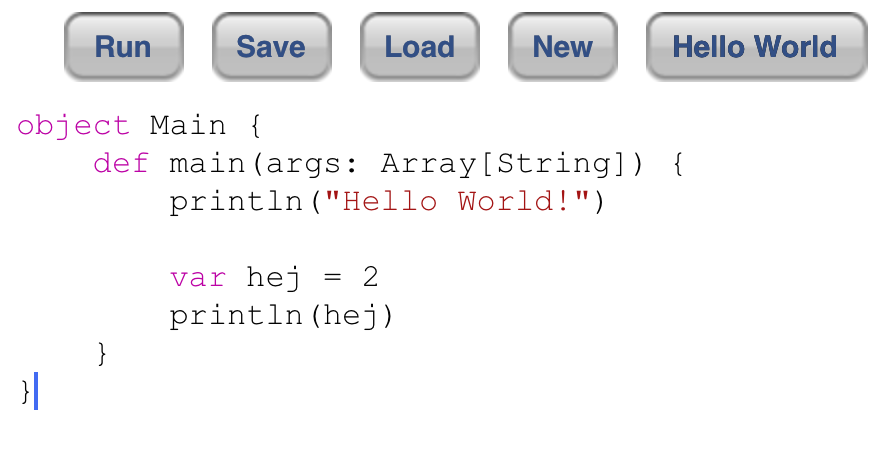
\includegraphics[width=80mm]{diagrams/CodeToGo_screenshot.PNG}
	\caption{The upper right corner of an example Scala program in CodeToGo.}
\label{fig:CodeToGo_screenshot}
\end{figure}

The most severe usability problem for CodeToGo is the low degree to which the user is able to recover from errors\,\cite{nielsen1990heuristic}. 
If you have a syntax error in your code you will get a standard console compile error from the \url{ideone.com} server. 
This error contains the line number where your program failed, but when you dismiss the error you will have to remember this line number and manually count your way down to the line where the mistake was, as the editor does not display line numbers\,\cite{nielsen1990heuristic}.

The editor only has the aforementioned character selector as an accelerator for advanced users. Other than that there are no ways for users to improve when using the tool other than to learn to type faster on an iPad\,\cite{nielsen1990heuristic}.

Nielsen recommends that you follow the iOS platform standards so that the user does not have to put too much effort into learning how to use each app in a special way. Nielsen also recommends having undo support. CodeToGo does have undo support and follows the standard way of iOS, which is to shake the device. One could argue that shaking their iPad is not the most elegant way of allowing programmers to undo their typing, so in this case following the standards is not necessarily what makes for the best user experience on a mobile programming interface.

\paragraph{Takeaways}
\begin{itemize}
	\item \textbf{Ta-1}: Do not assume that a virtual keyboard is as usable as a physical one\,\cite{nielsen2013mobile}. The touch interface has potential if you design your user experience to take advantage of it, but if you chose to ignore its potential/limitations you will have lower usability\,\cite{nielsen1990heuristic}.
	\item \textbf{Ta-2}: You need accelerators for users to become faster and more comfortable with the interface\,\cite{nielsen1990heuristic}. An accelerator could, for example, be auto completion and/or static checking.
	\item \textbf{Ta-3}: Undo support is essential for usability\,\cite{nielsen1990heuristic}, but shaking the device is probably not the right input method.
\end{itemize}

\subsection{Textastic}
\label{subsub:Textastic}
Like CodeToGo, Textastic aims to be a general purpose programming editor, and as such supports many popular programming languages. Unlike CodeToGo, however, it does not support any way to run your code (besides manually copying your program to a computer and running the code there). Textastic is interesting due to an interface component that is not seen in CodeToGo.

\begin{figure}
	\centering
		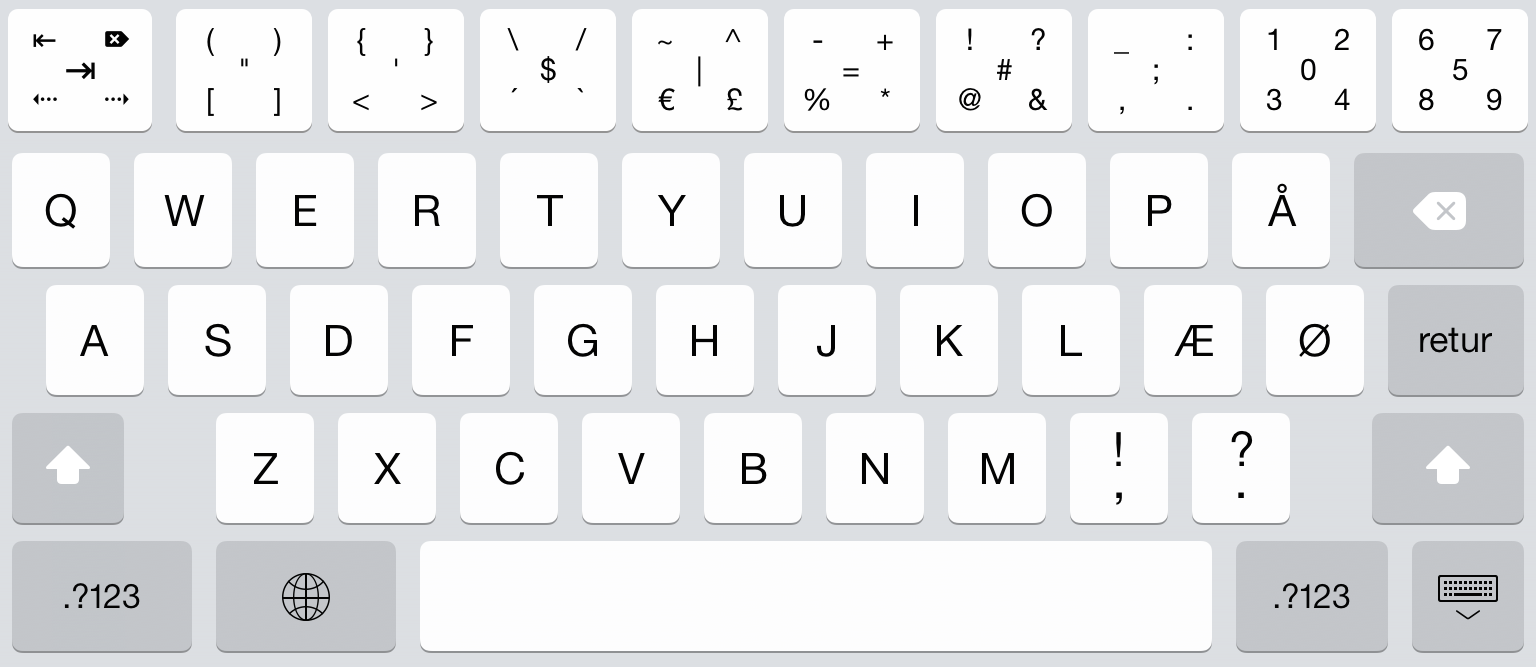
\includegraphics[width=110mm]{diagrams/textastic_keyboard_screenshot.png}
	\caption{The Textastic keyboard with special characters easily accessible.}
\label{fig:textastic_keyboard_screenshot}
\end{figure}

Textastic uses a shortcut bar that can be seen in Figure~\ref{fig:textastic_keyboard_screenshot}. This bar allows quick access to commonly used characters, that would otherwise be hard to get to with the virtual keyboard. To select a special character a user tap and hold your finger on the specific button and swipe towards the character that is needed. 

The biggest problem with Textastic is that you have no way of knowing whether your code will run or not\,\cite{nielsen1990heuristic}.\ On a computer, this would not be as big of a problem, in fact many programming editors do not analyze a program's semantics; instead, they rely on other software to run the code. This is much harder on a device such as an iPad, where multitasking is not as prevalent. The text editing interface is very reminiscent of none-touch GUI text editors.

\paragraph{Takeaways}
\begin{itemize}
	\item \textbf{Ta-4}: The solution Textastic has come up with for quickly accessing a large collection of symbols is the most intuitive we have seen.
	\item \textbf{Ta-5}: It is not enough to have a good editing interface, if such a basic issue as running your code is unaddressed.
\end{itemize}


\subsection{Raskell}
\label{subsub:Raskell}
Raskell is a Haskell editor for the iPad and a part of the UI can be see in Figure~\ref{fig:Raskell_screenshot}. It is based on the Hugs implementation of Haskell 98, and includes the ability to interpret your programs locally. The text editor itself is inspired by Vi, featuring many of the same keyboard commands. When you have written your program, you can load it into the interpreter, which gives you a read–eval–print loop (REPL), letting you test out your program. Raskell supports syntax highlighting for Haskell, and features most libraries for Hugs, but does not have auto completion.

The text editing itself works well, but a lack of auto completion and snippets mean you will be using the virtual keyboard to a large extent, which is generally a problem according to Nielsen\,\cite[pp. 76]{nielsen2013mobile}. 

\begin{figure}
	\centering
		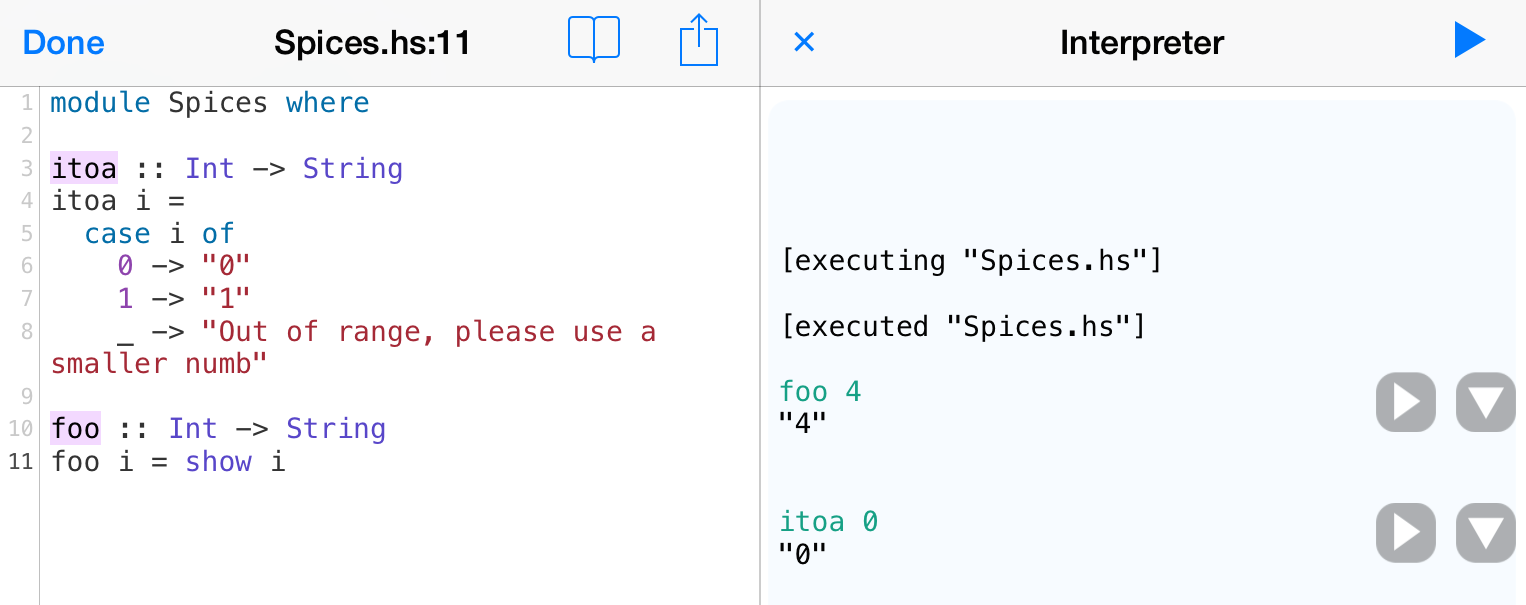
\includegraphics[width=110mm]{diagrams/Raskell_screenshot.png}
	\caption{The top of the Raskell environment with code editing to the right and a REPL to the
	left.}
\label{fig:Raskell_screenshot}
\end{figure}

Apart from this issue, the edit-compile-test loop is flexible and efficient. Especially compiler errors are handled in an elegant way, letting the user recover from syntactical errors\,\cite{nielsen1990heuristic}. If a compile error occurs, the user is presented with a split-screen view showing the error and a line number. The REPL is also extremely useful for trying out parts of your program.

Compared to CodeToGo, the Raskell development flow is quicker. This may be due to the local interpreter that evaluates your Haskell code as opposed to the network based approach CodeToGo takes.

\paragraph{Takeaways}
\begin{itemize}
	\item \textbf{Ta-6}: A good edit-compile-test loop greatly improves the development flow.
	\item \textbf{Ta-7}: A solid way to recover from syntax errors is essential to a good development experience\,\cite{nielsen1990heuristic}.
\end{itemize}

\paragraph{}

All three editors in this section have one main problem: The heavy reliance on the virtual keyboard. Also, only using one type of touch-gesture (the single tap) seems like a wasted opportunity.
According to Nielsen, it is important to optimize your solution for the touch
interface and not simply convert an existing desktop interface\,\cite[p 26, p
41]{nielsen2013mobile}.
One last issue that all of the above editors have in common is the lack of auto completion and user accelerators in general.

\section{Structural, Touch-Based Editors}
In this section we look at structured editors, which are different from the previously mentioned editors in that the editors are cognizant of the underlying structure of the program, the abstract syntax tree (AST). The user more or less directly manipulates this AST\@.

\subsection{Lisping}
\label{subsub:Lisping}
Using the Scheme dialect of LISP you can program and execute code right on your iPad with Lisping. The idea is to take advantage of the close proximity between the abstract syntax tree and source syntax of LISP to edit code in a structured way. The programmer is actually almost manipulating the abstract syntax tree directly instead of having to type in every single character of every single line. While other iPad solutions run code on an external server, Lisping runs locally using a Scheme interpreter written in C, called TinyScheme. Lisping has been written with usability in mind\,\cite{lisping}: 

``Textviews and virtual keyboards aren't the only option for coding on iOS\@. Editing source code character by character is a concept wedded to the keyboard and it is not necessarily the best option for a device with no keyboard.''

Lisping is also a touch-based programming editor with support for multiple types of gestures, but it is the fact that it is structured that makes it interesting to our study.

We are fairly experienced programmers with only little knowledge of the Scheme language and it's syntax, and we had a hard time understanding and using Lisping. The underlying TinyScheme interpreter most often gave us “Error Unknown” compiler messages even though we were writing examples straight from the Scheme website. Not being able to pinpoint what was syntactically wrong with the written code and recover from that error was a major problem, as stated by Nielsen's ninth heuristic\,\cite{nielsen1990heuristic}.

The editor supports a range of touch gestures that are not immediately obvious to the user. Low memorability is generally a problem with touch gestures as described by Nielsen\,\cite[p. 141]{nielsen2013mobile}. In Lisping, you have to open the Lisping guide in the upper right corner and read through 6 pages of a PDF document to familiarize yourself with these gestures. This is a memorability problem\,\cite{nielsen1990heuristic}.

As can be seen in Figure~\ref{fig:Lisping_screenshot}, there are also several buttons on the bottom of the UI\@. 
These are all icons and except for the delete and edit ones, they have no standard meaning in iOS or are used differently from the standard meaning. 
The undo button is e.g.\ a backwards-pointing triangle which could be interpreted to mean “Back” in iOS\@.
Given the fact that the user has no chance of remembering all these non-standard icons, they clearly violate the ``Recognition rather than recall'' and ``Consistency and standards'' usability guidelines\,\cite{nielsen1990heuristic}. 

\begin{figure}
	\centering
		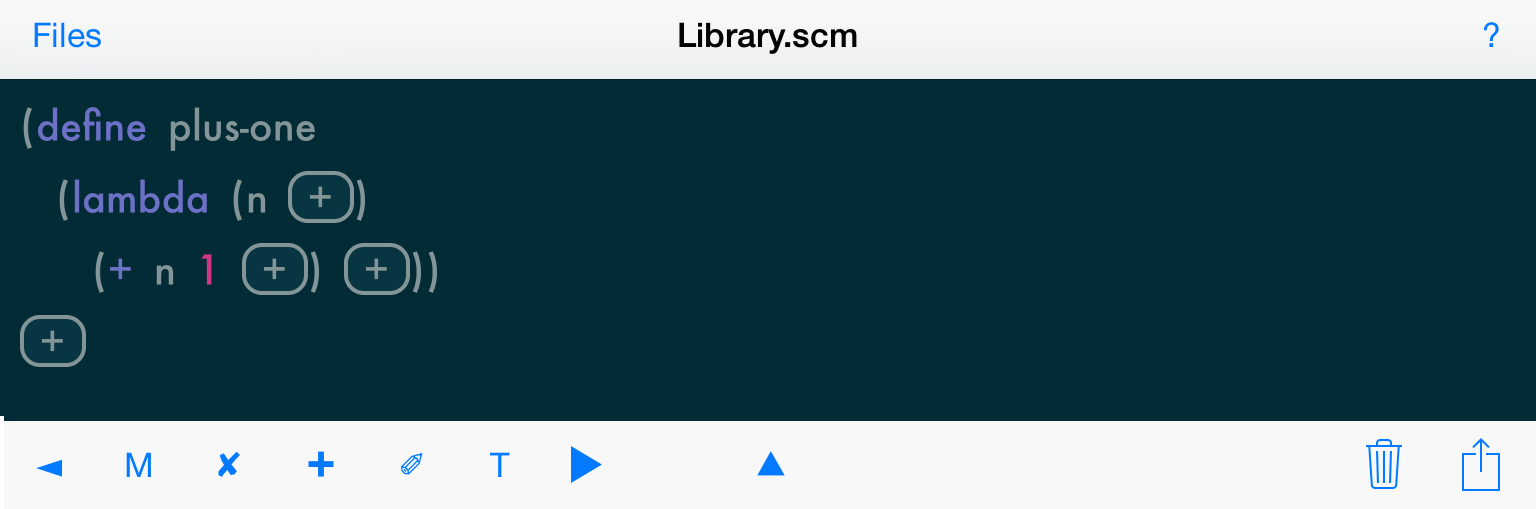
\includegraphics[width=110mm]{diagrams/Lisping_screenshot.png}
	\caption{A cropped screenshot of the Lisping interface, where the bottom
	toolbar consists of a range of non-standard icons and the program is filled
	with [+] buttons}
\label{fig:Lisping_screenshot}
\end{figure}

Furthermore, these icons are all located close to each other and potentially a whole screen's length away from where the user's attention is supposed to be when programming --- that is, on the code. All but two of the actions that these icons perform can be triggered with gestures performed on the source code. We see this as a incomplete attempt on providing accelerators for the expert user.

The problem with these gestures is that they are uncomfortable and cumbersome to use. To select an expression to edit or run in the REPL, the user must ``reverse pinch'' the text. This is a non-standard way of highlighting text in iOS and it feels very awkward and unresponsive not to mention that it gets painful to do after three to four times. It is even straining to perform normal tap gestures due to the small size of all the expressions in the editor.

The final usability problem we discovered with Lisping was the amount of [+] buttons inlined in the code. These buttons are supposed to indicate that an expression can be added there, but what they also do is make the code much harder to read.
In Figure~\ref{fig:Lisping_screenshot} we have a fairly simple program with
only three [+] buttons. This becomes more severe when the program grows.

\paragraph{Takeaways}
\begin{itemize}
	\item \textbf{Ta-8}: The error messages from the compiler/interpreter should indicate where in the code the syntax errors have occurred. Simply presenting ``Unknown Error'' is frustrating for the user.
	\item \textbf{Ta-9}: It should not be necessary to add a PDF document with instructions to how the gestures and buttons work. It should be immediately recognized by the user because it is all presented according to the platform standards. This serves as a reminder that the overuse of clever gestures harms the user experience.
	\item \textbf{Ta-10}: Littering a structured editor with [+] (add) buttons, to indicate that expressions can be added at these positions, is not a good idea. While a good alternative for this solution is hard to come up with we should try to design a different way.
\end{itemize}

\subsection{Eastwest}
\label{subsub:Eastwest}
Even though Eastwest is not a touch-based editor, we have included it in this section as it is a structured editor. 
While it is more of an experiment than a fully featured editor, we find it very interesting. It is an editor for a functional language that allows the user to ``fill in holes'', i.e.\ fulfill goals of a program from a popup. The context appears right under the goal and thus works as a well-placed auto completion tool. We have been unable to complete a heuristics evaluation of Eastwest, as we were unable to install it on our computers. Several videos are available, though, and it is interesting to see how functional data types are being defined and functions are being built in a structural way.

\paragraph{Takeaways}
\begin{itemize}
	\item \textbf{Ta-11}: Having a popup close to the goal makes for quick and easy access. The better that popup is at guessing the right thing for the goal, the faster the tool will seem.
	\item \textbf{Ta-12}: Eastwest is a good indication that functional languages work well in a structured editor.
\end{itemize}


\subsection{TouchDevelop}
\label{subsub:TouchDevelop}
TouchDevelop allows developers to make touch and accelerometer enabled games for any device with a web browser by providing a web app. It is generally meant as a way of getting children interested in programming, and the language has been specially designed for this purpose and works hand in hand with the development platform to provide a good experience for touch devices.

TouchDevelop displays a large auto completion area along the bottom of the interface, which shows relevant suggestions from the context. 
This means that you rarely have to type characters into the editor. 
Variable names are automatically generated at the push of a button.
Figure\ref{fig:TouchDevelop_screenshot} shows a sample program drawing a
turtle and a simple triangle pattern.

\begin{figure}
	\centering
		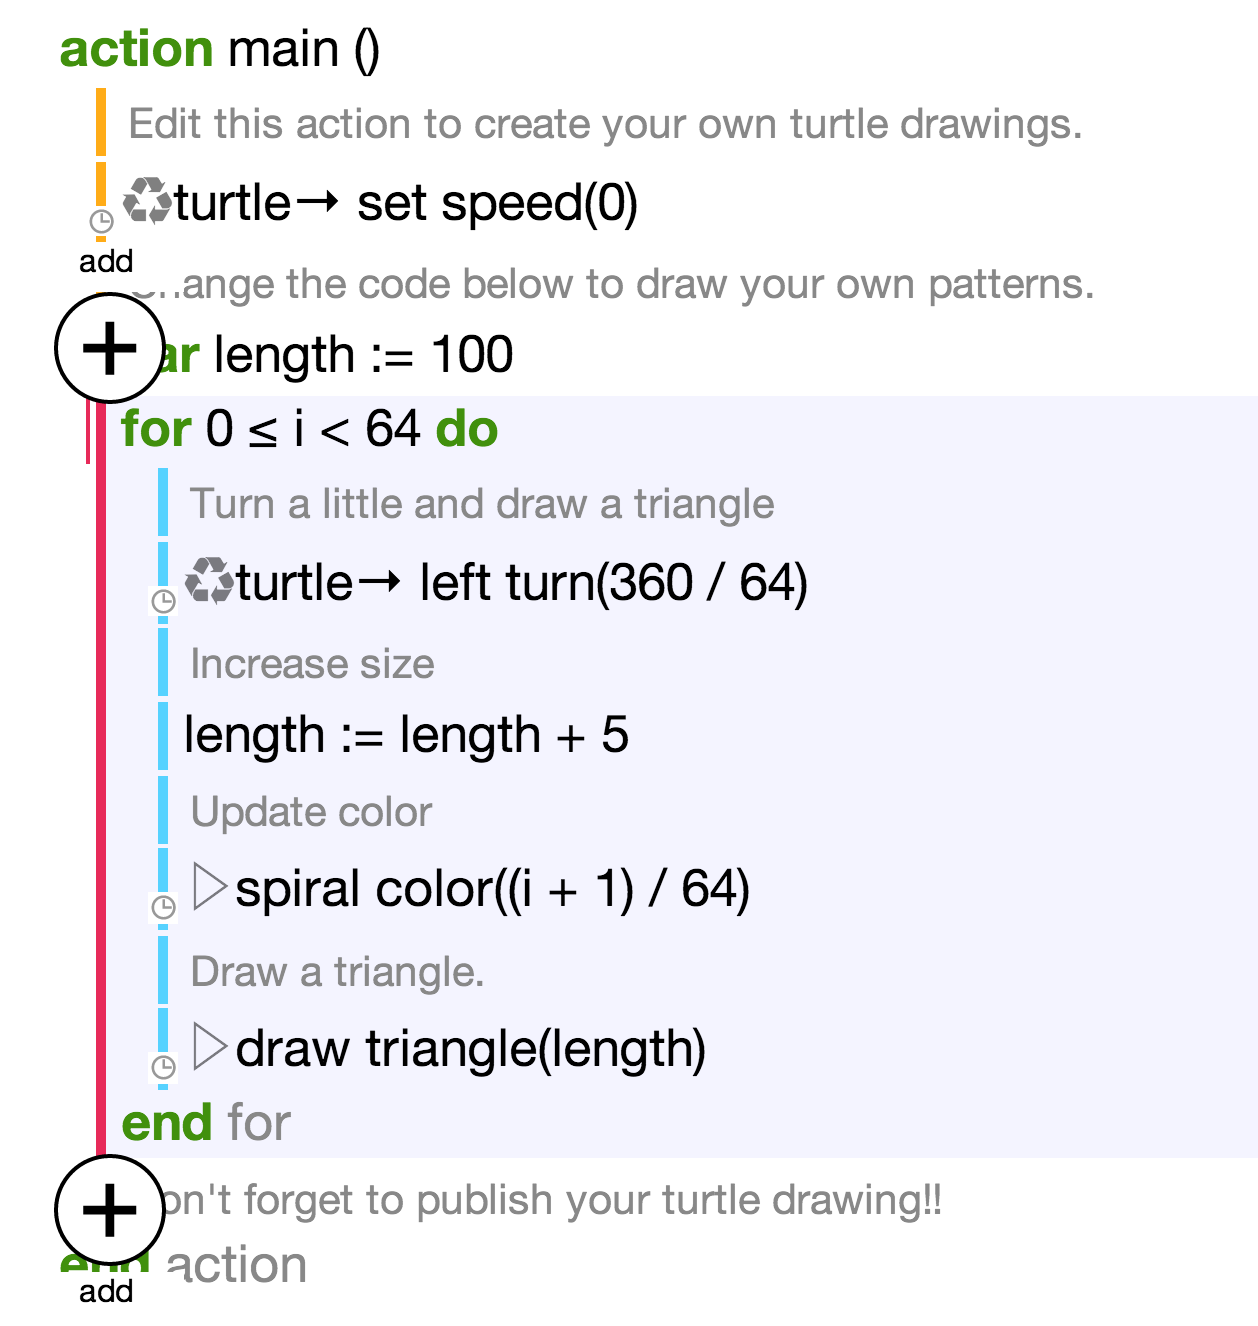
\includegraphics[width=80mm]{diagrams/TouchDevelop_screenshot.png}
	\caption{A screenshot of the Turtle Triangle Spiral sample from
	TouchDevelop\,\cite{TouchDevelop:TurtleTriangleSpiral}}.
\label{fig:TouchDevelop_screenshot}
\end{figure}

The first thing you notice as an experienced programmer is how the TouchDevelop language looks like modern imperative languages like C\# and Java, and this recognizability enabled us to get started with the platform right away. 
To educate new users there is a long tutorial that guides you through your first game. 

Even though TouchDevelop works on all touch devices that have a web browser it is not really optimized for other gestures than the standard single tap gesture that works on all platforms.

To fit more code on the screen and create a better programming overview, TouchDevelop uses a rather small font for the code you write. 
When you tap the line of code you wish to edit, that statement is enlarged and you can relatively easily move the cursor around. 
Additionally, buttons appear to insert new lines above and below the selected segment. 
This design is minimalistic and controls only show up when you need them\,\cite{nielsen1990heuristic}.

The auto completion area that is presented for selecting method calls and objects from is convenient when it presents you with just what you needed, but in most cases you find yourself struggling to find just that.
In these cases one must search using the virtual keyboard.
When filling out a hole in the program, the editor does not seem to narrow down the possibilities, as it displays options that would result in obvious type errors.

The user experience of TouchDevelop suffers from the fact that it is a web app written with no specific platform in mind. The biggest annoyance is when you want to move the cursor. This is clumsy on the iPad and often requires that you use buttons.

\paragraph{Takeaways}
\begin{itemize}
	\item \textbf{Ta-13}: To have a contextual overview can speed up the tasks of programming just as we saw with Eastwest.
	\item \textbf{Ta-14}: The type system of the TouchDevelop object oriented programming language is not ideal if you want to expose a context for the user to pick from. The type system simply can't narrow down the possibilities efficiently.
	\item \textbf{Ta-15}: Using a smaller font for code that is not in focus is a clever way to create a better overview for the user.
	\item \textbf{Ta-16}: There is a clear difference between the feel of a web app like TouchDevelop and a native app like Lisping.
\end{itemize}

\paragraph{}

As we have learned, it is of paramount importance to have as little use of the virtual keyboard as possible, and adopting the structured approach together with the strong type system of Idris might be able to provide just that.

\section{Visual Programming Languages} % (fold)
\label{sub:visual_programming_languages}
In this section we will investigate three editors with visual components.
It is possible that a more visual approach will work well on a touch-based interface, so even though Idris is not a visual language at all, we might find elements from these editors that our applicable to our design.

\subsection{LabVIEW}
\label{subsub:LabVIEW}
LabVIEW is a development environment featuring the G VPL which is designed for dataflow programming and uses the popular ``boxes and wires'' abstraction, with boxes performing various functions, and wires leading data between the boxes.
LabVIEW also lets users combine simple widgets to build GUI programs, using the G language for logic.
It is widely used in the scientific community, especially to work with data collected from sensors, and is often referenced in articles on VPLs\,\cite{Green96usabilityanalysis,DBLP:journals/ijmms/PetreB99}.
As such, we find it to be a good representative of this style of VPL\@.
Figure~\ref{fig:LabVIEWGettingStarted} shows a simple example of calculating a
triangle's area.

\begin{figure}[h]
\centering
\includegraphics[width=110mm]{diagrams/LabVIEW_screenshot.png}
\caption{A simple LabVIEW program from the tutorial\,\cite{LabVIEW:GettingStarted}}.
\label{fig:LabVIEWGettingStarted}
\end{figure}

While complex programs in G can be initially overwhelming to even experienced programmers, Whitley and Blackwell\,\cite[p. 445]{WHITLEY2001435} show that seasoned LabVIEW programmers prefer the visual syntax to their favorite textual language. Furthermore, the participants of the study found LabVIEW to be an effective tool, and highly rated the visual aspects of the
editor\,\cite[pp.
466]{WHITLEY2001435}.

\paragraph{Takeaways}
\begin{itemize}
	\item \textbf{Ta-17}: One interpretation of Whitley and Blackwell's findings\,\cite{WHITLEY2001435} is that although LabVIEW can be hard for programmers not used to the visual syntax, the higher learning curve pays off in the long run.
	\item \textbf{Ta-18}: The ``boxes and wires'' approach is good at indicating structure and could maybe be transfered to a more general purpose language.
\end{itemize}


\subsection{Scratch}
\label{subsub:Scratch}
Scratch is a VPL designed to be easy for beginners to use, facilitating the development of simple audio/visual programs. It is implemented as a web app, and features built-in tutorials, tips and help.
The language is built around a scene containing sprites. A scene can have multiple sprites, and each sprite can be governed by multiple scripts written in the Scratch visual language. The language itself consists of blocks of different shapes, colors and sizes. Scratch does not use the dataflow paradigm, as LabVIEW does. Instead, one programs by snapping blocks together. As can be seen from Figure~\ref{fig:ScratchProgram}, the blocks have different shapes, and only complementing shapes can be put together. Color is used to differentiate types of blocks.

\begin{figure}
	\centering
		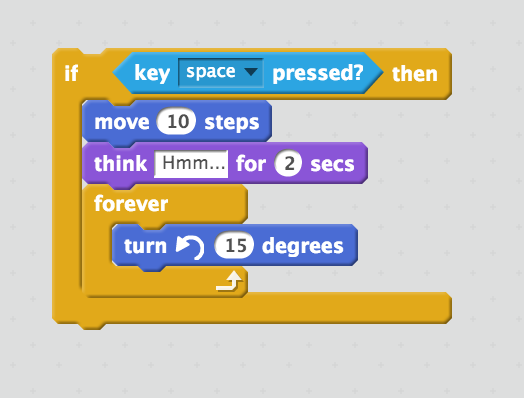
\includegraphics[width=60mm]{diagrams/ScratchProgram.png}
	\caption{A simple Scratch program that moves and spins the sprite if the space button is pressed.}
\label{fig:ScratchProgram}
\end{figure}

A wide range of solutions based on or similar to Scratch have been made over the years\,\cite{hosick2014}, but one is, in particular, interesting to us as it is a port of Scratch to the Apple iPad. It is called Hopscotch\,\cite{hopscotch} and generally does exactly what Scratch does just by incorporating two types of simple touch gestures.

The most interesting part of Scratch is the visual language itself.
Use of different colors for different types of elements (control structures, data management, input), along with different shapes for showing which elements can be combined makes it very easy to discriminate between different components.
Symbols are used in a semantically immediate way in some places, such as an arrow pointing back to the start of a loop. 
Complexity management is a problem for Scratch, as there does not seem to be a way to define new functions; each script is composed of exactly one function, and scripts cannot access anything from other scripts.
This means functions can become very long and unwieldy.
Scalability in VPLs has been explored in depth by Green and Petre\,\cite{green1992visual}.

\paragraph{Takeaways}
\begin{itemize}
	\item \textbf{Ta-19}: When designing a visual syntax, making it visually obvious which elements go together greatly increases the ease of learning.
	\item \textbf{Ta-20}: Using colors and shapes to differentiate elements is very important in a visual language.
	\item \textbf{Ta-21} Complexity management is hard with visual languages\,\cite{green1992visual}.
	\item \textbf{Ta-22}: Use all the aspects of visual expressiveness when designing a visual language, e.g.\ shape, color, texture, position, etc.
\end{itemize}

\subsection{Epigram}
\label{subsub:Epigram}
The Epigram\,\cite{mcbride2005epigram} language is a functional and dependently typed language made by Conor McBride, which aims to let the programmer create compiler certified proofs using intuitionistic logic.
It is not a traditional visual programming language, but it has been put in this category due to its 2D syntax.
Especially the syntax of the data type specification is interesting.
In Epigram, defining data is done in a more visual way than newer dependently typed languages. 
It is accomplished by imitating the standard way of writing inference rules.
As can be seen in Figure~\ref{fig:epigram_data}, the definition of e.g.\ a data type is split into three lines and its 2D syntax almost resembles ASCII art. 

\begin{figure}[htbp]
	\centering
	
	\lstinputlisting[firstnumber=1,basicstyle=\ttfamily\scriptsize]{code/epigram_data}
	\caption{The natural numbers defined in Epigram}
\label{fig:epigram_data}
\end{figure}

While it has not been possible to get a version of Epigram working for any sort of test, we are interested in how this way of expressing data types could benefit the user in a more structured editor, that does not require the user to maintain ASCII art, but still displays the program in a more visual way.

\paragraph{Takeaways}
\begin{itemize}
	\item \textbf{Ta-23}: The more visual way of writing data types could be more intuitive for people used to reading that sort of notation. This goes well with Nielsen’s ``Match between system and the real world''-heuristic.
\end{itemize}

\paragraph{}

While we think a more visual way of programming might be a good fit for a touch-based interface, the issues with complexity management and the high learning curve make us wary.
Instead of a completely visual editor, it might be possible to take certain elements to produce more readable programs. 
Especially the 2D data syntax from Epigram seems interesting.

The Epigram editor was also structured, but we were unable to obtain a
version of it.

% subsection visual_programming_languages (end)

\section{Existing Solutions Overview}
% Please add the following required packages to your document preamble:
% \usepackage{multirow}
% \usepackage[table,xcdraw]{xcolor}
% If you use beamer only pass "xcolor=table" option, i.e. \documentclass[xcolor=table]{beamer}

\begin{table}[ht]
{\renewcommand{\arraystretch}{2}%
\begin{tabularx}{\textwidth{}}{|c|X|c|c|c|}
\hline
	& \textbf{Description}
	& \textbf{Touch-based}                                              
	& \textbf{Visual syntax}                          
	& \textbf{Stuctured editor} 
\\ \hline
	\textbf{CodeToGo} & & \cellcolor[HTML]{B6D7A8}{\color[HTML]{9AFF99} }                  & & \\ \cline{1-1}
	\textbf{Textastic}  & \multirow{-2}{*}{
	Textual iPad env.
	} & \multirow{-2}{*}{\cellcolor[HTML]{B6D7A8}{\color[HTML]{9AFF99} }} & \multirow{-2}{*}{}                              & \multirow{-2}{*}{}                                                   
\\ \hline
	\textbf{Raskell}      & 
		Mobile Haskell & \cellcolor[HTML]{B6D7A8}{\color[HTML]{9AFF99} } & &                                                               
\\ \hline
	\textbf{Lisping}      & 
		Mobile Lisp & \cellcolor[HTML]{6AA84F} & & \cellcolor[HTML]{B6D7A8}

\\ \hline
	\textbf{Eastwest}     & 
		Functional programming system with structured editor
		 & & & \cellcolor[HTML]{274E13}
\\ \hline	
	\textbf{TouchDevelop} & 
		Imperative language running as a web app
		 & \cellcolor[HTML]{6AA84F} & & \cellcolor[HTML]{B6D7A8} 
\\ \hline		
	\textbf{LabVIEW}      & 
		Visual data flow programming & & \cellcolor[HTML]{38761D} & \cellcolor[HTML]{6AA84F}
\\ \hline
	\textbf{Scratch}      & 
		Beginner-friendly programming by dragging boxes
		  & & \cellcolor[HTML]{274E13} & \cellcolor[HTML]{274E13}
\\ \hline
	\textbf{Epigram}      & 
		Functional with Dependent Types & & \cellcolor[HTML]{6AA84F} & Unknown
\\ \hline
\end{tabularx}
}
\caption{Existing solutions overview. The darker the green the more the
emphasis on this aspect of the editor.}
\label{table:existing_solutions_overview}
\end{table}

In this section we have analyzed a range of existing solutions and for each reached a list of takeaways that we will use when determining the requirements for our design.

The current state of the art touch-based iPad apps either only use the single tap gesture, thus wasting a golden opportunity, or use several gestures without concern for the usability of them. 
The issue seems to be that they are all essentially manipulating text and that the standard text input UI elements on the iPad already support several gestures. 
If the app tries to incorporate too many gestures to manipulate the structure of these text fields there may be conflicts. 
Finding a solution to this problem is a major challenge.

We also discussed a few structured editors, where two of them support functional languages. 
Having the editor be cognizant of the underlying structure of the program seems to lessen the amount of typing the user has to perform on the virtual keyboard. 

Finally, a more visual approach might be appropriate, but several issues, such as complexity management issues, means special care must be taken.
Table~\ref{table:existing_solutions_overview} gives an overview of the existing solutions.
